\documentclass[a4paper]{report}
\usepackage[T1]{fontenc}
\usepackage[sfdefault]{biolinum}
\usepackage[french]{babel}
\usepackage{setspace}
\usepackage{tabularx}
\usepackage{graphicx}
\graphicspath{{assets/}}
\usepackage{wrapfig}
\usepackage{float}
\usepackage[headheight=13pt,top=3cm, bottom=2cm, left=1.5cm, right=1.5cm]{geometry}
\usepackage{fancyhdr}
\pagestyle{fancy}
\usepackage{hyperref}
\hypersetup{
    colorlinks=true,
    linkcolor=black,
    citecolor=black,
    filecolor=black,
    urlcolor=black,
}
\renewcommand{\headrulewidth}{1pt}
\renewcommand{\footrulewidth}{1pt}
\fancyfoot[L]{ENSIAS}
\fancyfoot[C]{\textbf{\thepage}}
\fancyfoot[R]{Année universitaire: 2020/2021}
\author{Kotbi Abderrahamane}
\date{Thursday, July 1st 2021}

\begin{document}

\begin{titlepage}
  \begin{center}
      \begin{figure}[!h]
          \vspace{- 2 cm}
          \hspace{ 0 cm}
          
\includegraphics[width=9em]{ensias.jpeg}
      \end{figure}
      \begin{figure}[!h]
          \vspace{- 3.34cm}
          \hspace{14cm}
          
\includegraphics[width=10em]{um5.jpeg}
      \end{figure}
  \end{center}

  \begin{center}
      \begin{center}
          \rule{0.9\linewidth}{1pt}
      \end{center}
      \vspace*{0.2cm}
      \noindent \hspace{ 0.3 cm }\Huge \textbf{Étude de l'architechture de l'entreprise AGRI}
      \begin{center}
          \rule{0.9\linewidth}{1pt}
      \end{center}

      \vspace*{0.5cm} \noindent \hspace{ -0.5 cm} \large
      \begin{figure}[H]
          \begin{center}
              
\includegraphics[scale=0.4]{archimate-image.png}
          \end{center}
      \end{figure}
  \end{center}
  \vspace*{0.5cm} \noindent \hspace{ -0.5 cm} \large
  \textbf{\emph{Préparé par: 
  \begin{itemize}
    \item[•] KOTBI Abderrahamane
    \item[•] EL-HAFI Abdessamade
\end{itemize}}}
  \raggedright{\rule{0.7\linewidth}{2pt}}\\
  \textbf{\emph{
          Encadré par:\\
          Pr. Salah BAINA
      }}
  \mbox{}\vfill
  \begin{center}
      \rule{0.9\linewidth}{1pt}\\
      \Large\emph{
          Filière Génie Logiciel\\
          Année universitaire: 2020/2021
      }
  \end{center}
\end{titlepage}

\newpage

\fancyhead[R]{\textbf{Table des matières}}
\fancyhead[L]{\hspace*{5cm}}
\tableofcontents

\newpage
\listoffigures

\newpage
\renewcommand{\listtablename}{Table des tableaux}
\listoftables

\newpage

\begin{doublespace}
  \chapter*{\centering Introduction}
  \addcontentsline{toc}{chapter}{Introduction}
L'architecture d'entreprise (AE) est une discipline qui permet de gérer
les approches conflictuelles au sein des organisations. Cette
discipline, consacrée tant au monde de l'informatique qu'à celui du
métier, introduit des normes pratiques dans les différentes unités et
départements afin d'optimiser l'utilisation des ressources
disponibles.Cette étude de cas illustre l'intérêt du langage de
modélisation ArchiMate pour le développement et la mise en œuvre de l'EA
chez l'entreprise Agri.AGRI est une entreprise specialiste dans la vente
des produits agricoles et cette étude illustre principalement les
couches centrales du langage ArchiMate appliquee a Agri comme example
ainsi que ses deux extensions : Motivation et implémentation et
Migration.

\chapter{Présentation de l'entreprise Agri}
\fancyhead[R]{\textbf{Chapitre \thechapter: Présentation de l'entreprise Agri}}
\fancyhead[L]{\hspace*{5cm}}

\section{Context général de l'entreprise Agri}

\begin{quote}
L'activité de la société AGRI consiste en la vente des produits
agricoles vers un ensemble de clients qui peuvent être soit des
distributeurs détaillants ou alors des particuliers. Elle est composée
de trois agences et un siège principal. Cette décomposition de
l'entreprise permet de bien cerner les tâches des agences et de siège.
Par conséquent, nous pouvons dégager les acteurs avec les quels ils
travaillent, les services offers par chacun parmi eux, et les
processuses englobés.Le tableau suivant résume les différents service
ainsi que ses procèdes , acteur at son département.
\end{quote}

\begin{table}[H]
\begin{center}
\begin{tabularx}{17.5cm}{|p{2.5cm}|p{7cm}|X|p{2cm}|}
\hline
Services & Procédés & Acteurs & Département \\
\hline
Vente & Vente: répondre aux commandes des clients, Facturation ,
Livraison au clients & Client, équipe vente & agence \\
\hline
Achat & Achat, Facturation & Fournisseur, Direction & siège \\
\hline
Facturation & Facturation des commandes & équipe de facturation &
siège \\
\hline
Comptabilité & Comptabilité & équipe de comptabilité & siège \\
\hline
Stock & gestion des stocks & équipe de stock & agence \\
\hline
Resource humain & gestion des resources humains & équipe de resources
humains & siège \\
\hline
\end{tabularx}
\caption{Title}
\end{center}
\end{table}
\section{Structure organisationnelle}

\begin{quote}
D'aprés la partie précédent nous avons retenu la conclusion suivante:

\begin{itemize}
\item
  L'entreprise Agri est composée en deux types de département:
\end{itemize}

\begin{itemize}
\item
  Agences ont une intéraction directe avec le client.
\item
  Siège représent le back-office et s'occupe plus des services de
  comptabilité, etc. Il communique également avec les fournisseurs.
\end{itemize}

\begin{itemize}
\item
  Chaque département est composée d'un ensemble des services.\\
  En prenant cela en consédiration, nous avons arrivés à réaliser le
  shéma suivant qui représente d'une manière exhaustive, mais claire,
  l'ensemble des services et les interactions que l'entreprise aura
  eventuellement avec son environement.
\end{itemize}
\end{quote}

\begin{figure}[H]
	\begin{center} 
		\fbox{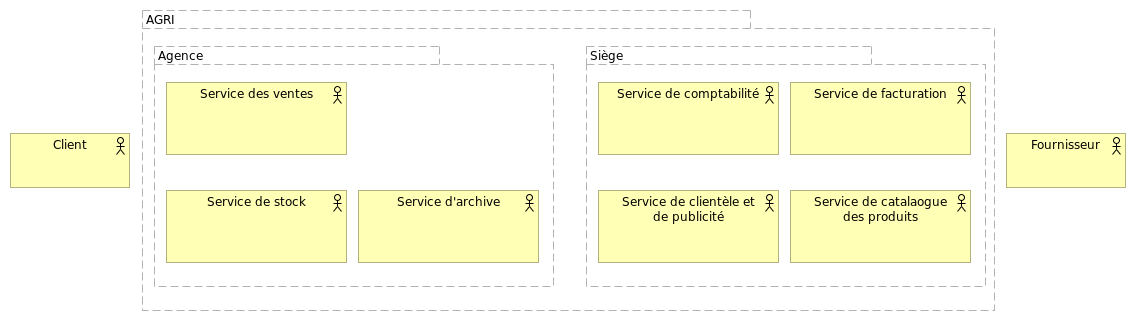
\includegraphics[scale=0.3]{id-ffaa0025f5024b42bb5c8eab10fc9707.png}}
		\caption{Title}
	\end{center}
\end{figure}

\section{Processes rescensés}

\begin{quote}
Dans la partie suivante on va essayer de comprendre comment la société
Agri gère sont travail. Donc, on va essayer de lister les processes
englobés dans son métier.Pour le faire, on va commencer par les
processes reliés au client, puis ceux de fournisseurs.
\end{quote}

\begin{quote}
\begin{itemize}
\item
  Le client est en générale intervient dans les services de ventes et
  d'aprés ventes, tels que la publicité. On peut comprendre plus
  concrétement les services qui doit servire ce dernier de schéma
  suivant:
\end{itemize}
\end{quote}

\begin{figure}[H] 
	\begin{center}
		\fbox{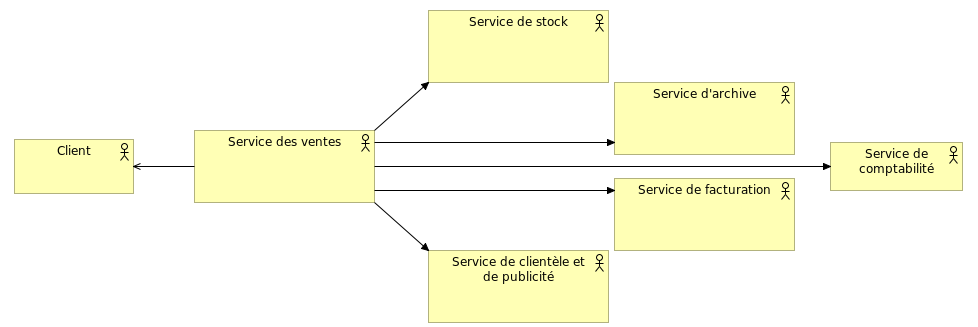
\includegraphics[scale=0.3]{id-b73f5c477dc542ca8680eaa522807b25.png}}
		\caption{Title}
	\end{center}
\end{figure}

\begin{quote}
On peut voire clairement ces processes d'aprés le schéma suivants:
\end{quote}


\begin{figure}[H] 
	\begin{center}
		\fbox{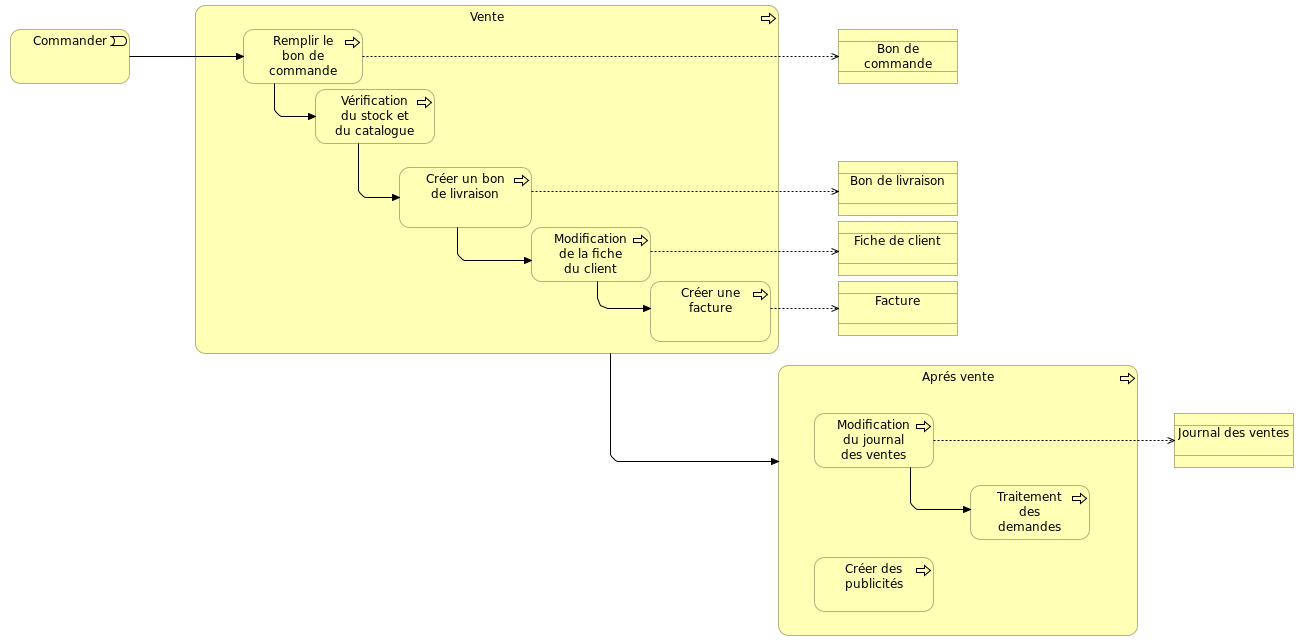
\includegraphics[scale=0.3]{id-b73f5c477dc542ca8680eaa522807b27.png}}
		\caption{Title}
	\end{center}
\end{figure}

\begin{quote}
\begin{itemize}
\item
  En ce qui concerne le fournisseur, ses interventions sont
  semèstrielles et ont comme objective la mise-à-jour de catalogue des
  produits:
\end{itemize}
\end{quote}

\begin{figure}[H] 
	\begin{center}
		\fbox{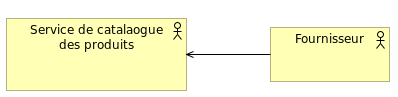
\includegraphics[scale=0.3]{id-b73f5c477dc542ca8680eaa522807b28.png}}
		\caption{Title}
	\end{center}
\end{figure}

\begin{quote}
Le schéma suivante montre ce processus de changement de catalogue:
\end{quote}

\begin{figure}[H] 
	\begin{center}
		\fbox{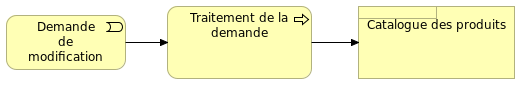
\includegraphics[scale=0.3]{id-b73f5c477dc542ca8680eaa522807b26.png}}
		\caption{Title}
	\end{center}
\end{figure}

\section{Problématiques de l'entreprise Agri}

\begin{quote}
Dans cette partie on va essayer de dégager les problémes que pose
l'architecture actuelle de l'entreprise Agri. Il est trés important de
bien cibler les vrais problèmes de la société. Certes, ces derniers sont
en général en relation avec le gaspillage des ressources, la structure
non-optimale des services de l'entreprise. Mais, il est tellement
important aussi de penser à des problèmatiques d'innovation qui permet à
l'entreprise à garder sa compétitivité pour le long terme.
\end{quote}

\begin{itemize}
\item
  Les problèmes dues à la gestion des ressources:
\end{itemize}

\begin{itemize}
\item
  Le premier poblèmes qu'on peut voire clairement est le problème de
  gaspillage des papiers. Beacoup de documents se partagent en beaucoup
  d'exemplaire entre les différents services. Ceci demeure une méthode
  fastidieuse pour le traitement et le stockage des données. En plus
  parmis ces documents on voit que le bon de commande qui doit être
  rempli par le service de vente est une solution non efficace. Il est
  mieux de penser à des solutions de genre \emph{serve yourself}. Car
  d'une part, le remplissage des commandes par des agents est un
  gaspiallge des papiers et des ressources humains, et d'autre part ceci
  peut donner une experience non-satisfaisante pour le client.
\item
  Sur la même longueur d'onde, on peur remarquer que les données qui
  bascules entre les différents services imposent plusieurs problèmes
  car la données est par tout et on doit passer parfois par plusieurs
  services avant d'obtenir l'information en question. Ceci implique
  qu'il faut aussi repenser l'architecture des services de l'entreprise
  pour en bien tirer profit.
\item
  Sur un plus grand échelle, l'information par fois prendre un temps
  pour faire la mise-à-jour. À l'instar de le journal des ventes qui
  nécessite un délait de 24 heurs avant qui soit mise-à-jour.
\end{itemize}

Les problèmes pour l'innovation:

\begin{itemize}
\item
  Agri générer plusieurs données sur ces clients et ventes qui ne sont
  pas stockée puis utilisée pour les analyser et en tirer des
  conclusions qui peuvent aider à prendre des discisions stratégiques.
  Par exemple Agri peut penser a utilisé ses données pour augmenter la
  vente d'un tel produit ou pour des fins de marketing et publicitaires.
\end{itemize}

\chapter{Motivations pour la transformation digitale}
\fancyhead[R]{\textbf{Chapitre \thechapter: Motivations pour la transformation digitale}}
\fancyhead[L]{\hspace*{5cm}}

\begin{quote}
L'entreprise Agri peut penser à des solutions pour remédier les
problèmes cités précédement, afin d'optimiser ses processes de ventes,
et par conséquent, augmenter le chiffre d'affaire. En effet, il faut
prendre en considération trois pilliers essentiels: le client, le
produits, et la vente. En ce sens, il faut satisfaire le client en lui
proposant un service et un produit de qualité, et par la suite augmenter
les profits et minimiser les coûts.
\end{quote}

\begin{figure}[H] 
	\begin{center}
		\fbox{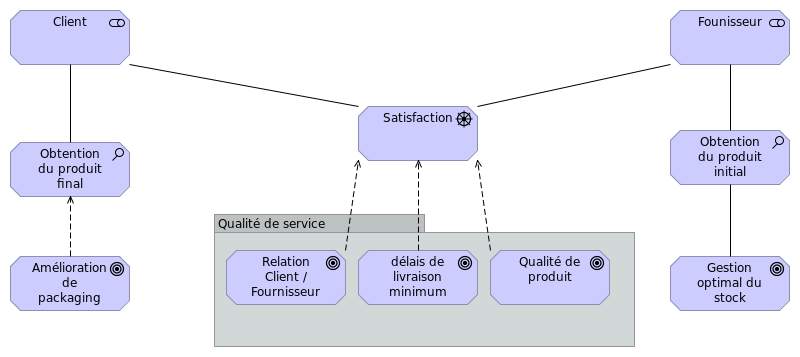
\includegraphics[scale=0.3]{id-0f11c567da544c39bef6a790b752afbc.png}}
		\caption{Title}
	\end{center}
\end{figure}

\chapter{Vision cible pour l'entreprise Agri}
\fancyhead[R]{\textbf{Chapitre \thechapter: Vision cible pour l'entreprise Agri}}
\fancyhead[L]{\hspace*{5cm}}

\section{Mise en œuvre et migration}

Les problématiques citées précédemment nous pousse à repenser à des
solutions stratégiques qui peuvent améliorer la chaine de vente de
l'entreprise Agri. En effet l'intégration d'un système d'information
pourra être une partie intégrante de la stratégie de l'entreprise qui
permettra de surmonter ses difficultés pour gérer efficacement la
traçabilité entre les briques d'architecture du système et les besoins
exprimés à l'origine du projet; et encore plus à justifier des décisions
d'architectures vis-à-vis de ces attentes. \\
En prenant en considération des améliorions au niveau de l'architecture
d'Agri, celle-ci dorénavant possède un GPS qui lui guide dans ses choix
au fur et à mesure des différentes étapes à traverser, en réduisant
l'incertitude et en fournissant les informations nécessaires à la bonne
évaluation des différentes possibilités.

Au niveau métier, cette amélioration va permettre à l'entreprises de
définir sa stratégie et de clarifier sa vision, mission et objectifs
grâce à l'évaluation des facteurs de changements tel que des facteurs
métiers ou de régulation. Elle permet ensuite de planifier les capacités
métiers nécessaires pour atteindre les objectifs définis, et de définir
une stratégie et une tactique pour chaque objectif. \\
Une fois les capacités métiers planifiés, les directions informatiques
vont pouvoir planifier les fonctionnalités IT, les applications, les
technologies et l'infrastructure nécessaires pour pouvoir supporter les
métiers.

L'architecture d'entreprise améliorée fournit ainsi à Agri des feuilles
de route métier et IT claires qui laissent peu de place à l'incertitude.
Couplée à la gestion des risques métier et IT, les améliorations qu'on
va présenter permet de réduire les risques liés à toute transformation
en évaluant leur impact et leur probabilité, et en mettant en place des
plans d'actions visant à réduire ces risques.

Le diagramme suivant propose comment nous pouvant mener à bien cette
Migration dans l'architecture de l'entreprise Agri.

\begin{figure}[H] 
	\begin{center}
		\fbox{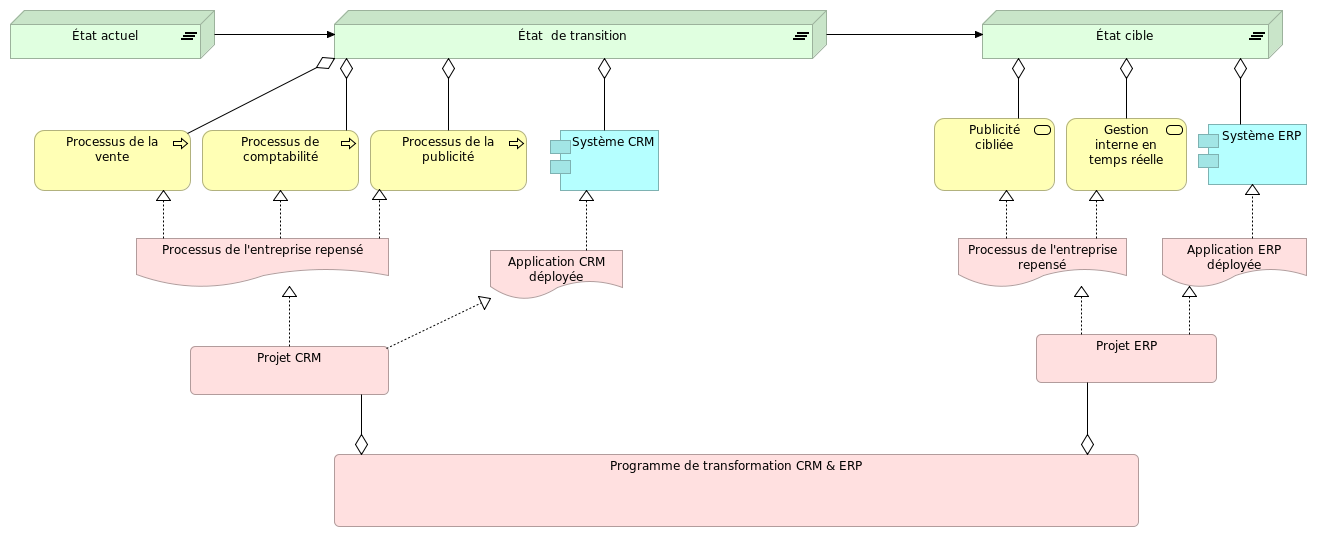
\includegraphics[scale=0.3]{id-1665e6d9cf6a447d9cd191be7c8da8e3.png}}
		\caption{Title}
	\end{center}
\end{figure}

\subsection{Architecture de l'entreprise cible}

\begin{quote}
Dans la partie suivante on va voire comment on peut bien améliorer le
métier de l'entreprise Agri en innovant son architecture.

\subsection{Vision d'adoption du CRM chez Agri}
\end{quote}

Agri peut penser à intégrer un CRM qui peut enregistrer et gérer chaque
contact et échange avec chaque client existant ou potentiel, sauvegarder
toutes leurs préférences, et suivre toutes leurs activités. Par CRM, on
entend soit la stratégie globale visant à mieux gérer ses relations avec
le client et dont l'objectif est d'augmenter les ventes et les profits,
en fidélisant les clients sur le long terme et en donnant priorité au
client pour lui offrir une expérience entièrement personnalisée et
fondamentalement meilleure ; soit la technologie qui permet de gérer ces
relations, en conservant et en organisant sur une seule plateforme les
données concernant chaque client, client potentiel ou lead et en
assurant le suivi de tous les échanges ou contacts entre l'entreprise et
ces clients.

Le diagramme suivant présente comment on peut penser à l'intégration du
CRM au sein de Agri.

\begin{figure}[H] 
	\begin{center}
		\fbox{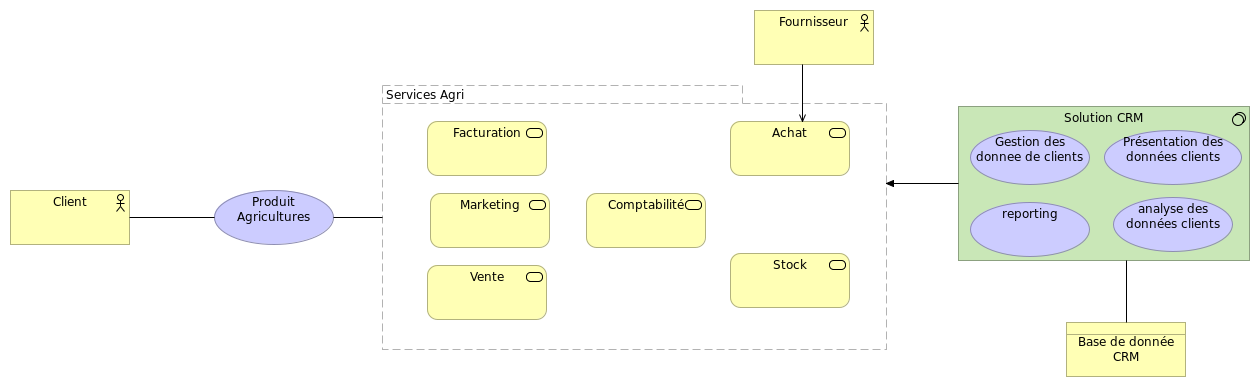
\includegraphics[scale=0.3]{id-ce6e1329804e4403a26757a131ad5358.png}}
		\caption{Title}
	\end{center}
\end{figure}

Lors de son séjour d'achat, le client génère assez de données intéressantes qui peuvent faire l'objet des input du CRM. En effet, le CRM peut aider à la gestion des clients, à la présentation des données clients ainsi qu'à faire des analyses et du reporting.

\subsection{Vision d'adoption d'un ERP chez Agri}

Une autre amélioration qu'Agri peut penser à mettre en œuvre est de
d'intégrer un ERP. Un ERP est une solution logicielle visant à unifier
le système d'information d'une entreprise en intégrant les différentes
composantes fonctionnelles autour notamment d'une base de données
unique. D'autre mot, un ERP est un système complexe qui demande du temps
à appréhender et mettre en place mais qui peut être extrêmement
profitable à la rentabilité d'une entreprise.

\begin{figure}[H] 
	\begin{center}
		\fbox{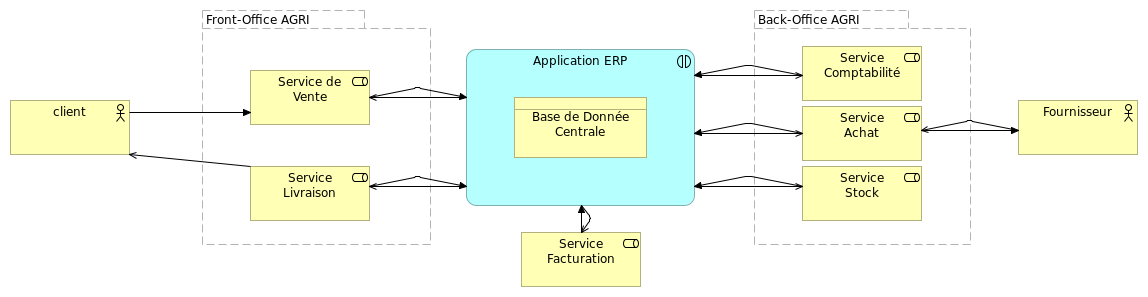
\includegraphics[scale=0.3]{id-81b3dfb862e64da1b0d0ff04d309d954.png}}
		\caption{Title}
	\end{center}
\end{figure}

La solution ERP présentée dans le schéma précédent se présente comme un système central partagé par tous les différents services. Cette connexion à un nœud central permet le partage des données et la mise en temps réel de différentes données.
Concrètement, lorsqu'une commande est demandée par le client le service de vente se lance pour vérifier que la quantité demandée est bien disponible dans le stock, l'accès à la base de donnée central permet dans ce cas de savoir les dernier donnée sur l'état de stock. Lorsque la commande est servie le service de stock mis à jour la nouvelle etat de stock.

\chapter{Outils de réalisation}
\fancyhead[R]{\textbf{Chapitre \thechapter: Outils de réalisation}}
\fancyhead[L]{\hspace*{5cm}}

\section{Présentation de l'outil ArchiMate}

\begin{figure}[H] 
	\begin{center}
		\fbox{
\includegraphics{archimate-logo.png}}
		\caption{Title}
	\end{center}
\end{figure}

ArchiMate fournit des outils pour aider les architectes d'entreprise à
décrire, analyser et visualiser les relations entre les différents
domaines de l'architecture d'une manière non ambiguë, similaire à ces
disciplines bien établies comme le génie civil ou le bâtiment et la
construction en utilisant des normes internationalement acceptées pour
décrire leurs conceptions.

ArchiMate est une technique de modélisation pour décrire les
architectures d'entreprise. Il présente un ensemble clair de concepts et
de relations entre les domaines d'architecture, et offre une structure
simple et uniforme pour décrire le contenu de ces domaines. Tout comme
un dessin d'architecture dans l'architecture classique du bâtiment
décrit les différents aspects de la construction et de l'utilisation
d'un bâtiment.

Les principaux avantages d'ArchiMate pour la modélisation de vos
architectures d'entreprise sont :

\begin{itemize}
\item
  Il s'agit d'une norme internationale et indépendante des fournisseurs
  de The Open Group, vous libérant du verrouillage des outils et des
  cadres spécifiques aux fournisseurs. Il y a un soutien actif du Forum
  ArchiMate de The Open Group.
\item
  Ses concepts et modèles bien fondés apportent de la précision. Il vous
  aide à vous éloigner de l'image des « images floues » de
  l'architecture.
\item
  C'est un langage léger et simple. Il contient juste assez de concepts
  pour modéliser l'architecture d'entreprise et n'est pas pléthorique
  pour inclure tout ce qui est possible.
\item
  Sa structure uniforme le rend facile à apprendre et à appliquer.
\item
  Il a des liens clairs avec les approches existantes pour des domaines
  d'architecture spécifiques tels que les logiciels ou les processus
  métier.
\item
  Plusieurs concepts d'ArchiMate ont été délibérément empruntés à
  d'autres langages tels que UML ou BPMN, pour fournir un pont facile.
\item
  Il ne prescrit pas de méthode de travail, mais il se combine
  facilement avec des méthodes existantes telles que TOGAF.
\item
  Il a été essayé et testé par de nombreuses organisations
  d'utilisateurs différentes et est soutenu par de nombreux consultants
  et outils logiciels.
\end{itemize}

\chapter*{\centering Conclusion}
\addcontentsline{toc}{chapter}{Conclusion}
L'étude de l'architecture de l'entreprise Agri incite l'esprit pour
avoir une vision globale de l'entreprise et saisit les éléments
essentiels de l'entreprise dans son environement, ses systèmes d'information et leur évolution. Dans ce sens, il est
important de voir une vision innovative pour la transformation de l'entreprise. L'étude de l'entreprise Agri en
particulier illustre comment le standard Open Group ArchiMate pour la
modélisation architecturale de haut niveau peut être utilisé pour analyser, concevoir et guider les processus de transformation
d'entreprise. Les modèles ArchiMate offrent une vue d'ensemble des processus métier et de leur
informatique sous-jacente, tout en omettant intentionnellement les détails de conception des
processus, des applications et de l'infrastructure technique. Le langage de modélisation ArchiMate se
concentre plutôt sur la structure globale de ces domaines et sur les relations entre eux. Cela
aide les parties prenantes, des dirigeants d'entreprise aux ingénieurs, à comprendre l'alignement
entre les composants tels que les processus métier et leurs applications de support.

\end{doublespace}
\end{document}
